\documentclass[twocolumn,10pt,dvipdfmx]{jarticle} 

\usepackage{resume}
\usepackage{amsfonts}
\usepackage{graphicx}
\usepackage{amsmath}
\usepackage{bm}
\usepackage{algpseudocode,algorithm}
%\usepackage{ascmac}
\usepackage{theorem}
\usepackage{latexsym}
\usepackage{theorem}
\usepackage{mathtools}
\usepackage{comment}
\usepackage{color}
\mathtoolsset{showonlyrefs=true}
\DeclareMathOperator*{\argmax}{arg\,max}
\DeclareMathOperator*{\argmin}{arg\,min}
\numberwithin{equation}{section}
\newtheorem{theorem}{定理}[section]
\newtheorem{lem}{補題}[section]
\newtheorem{proof}{証明}
\newtheorem{coro}{系}[section]
\renewcommand{\theproof}{}
\def\qed{\hfill $\Box$}

\date{平成30年2月7日}
\title{\Large Partition制約付き最小化ナップサック問題に対する3-近似アルゴリズム}
\classification{卒業研究発表会資料}
\organ{電気通信大学}
\department{情報理工学部 情報・通信工学科 情報数理工学コース}
\studentid{1411070}
\author{木村 優貴}
\laboratory{村松 正和}
\centeruid
\oneside

\begin{document}
\maketitle
\section{はじめに}
	本研究ではNP困難な問題に対するアプローチの中でも代表的手法である主双対法を用いて近似アルゴリズムの設計を行った.\par
	近似アルゴリズムとは,最適値に十分に近い目的関数値が得られるような解を求めるアルゴリズムである.
	近似アルゴリズムの中でも最適化問題の全ての入力に対して最適値の$\alpha$倍以内の値を持つ解を返すアルゴリズムを
	その最適化問題に対する$\alpha$-近似アルゴリズムと呼ぶ\cite{apx_des,apx_al}.この時の$\alpha$を近似率と呼ぶ.
	最小化問題に対しては$\alpha>1$であり,最大化問題に対しては$\alpha<1$となる.\par
	最小化ナップサック問題は,
	品物をナップサックに価値の総和をある需要以上に保ちつつ,詰め込む品物の重さの総和を最小化することを目的とする問題である\cite{apx_des}.
	この問題はNP困難な問題であることが知られており\cite{np_c},最適解の導出や近似アルゴリズムの設計が広く行われている.\par
	本研究は,この最小化ナップサック問題に対し新たな制約を加え,拡張した問題に対して制度保証のある近似アルゴリズムの提案を行う.

\section{Partition制約付き最小化ナップサック問題}
	集合$\mathcal{P}$を
	\begin{align}
		\begin{array}{ll}
			\mathcal{P} = \{P_1,\dotsc,P_m\} & \\ 
			\mathcal{P}\subseteq 2^V, |P_j|\ge 2 & \forall j\in\{1,\dotsc,m\}\\
			P_i\cap P_j = \emptyset & \forall i,j \in \{1,\dotsc,m\}(i\neq j)
		\end{array}
	\end{align}
	と定義し,
	以下の問題を考える: 
	\begin{subequations}
		\begin{align}
				\mathrm{min } & \displaystyle\sum_{j\in V}{c_jx_j}\label{mkppc_1}\\
				\mathrm{s.t.} & \displaystyle\sum_{j\in V}{a_jx_j}\ge b\label{mkppc_2}\\
							& \displaystyle\sum_{j\in P}{x_j}\ge 1 \qquad\qquad \forall P\in \mathcal{P}\label{mkppc_3}\\
							& x_j \in \{0,1\} \qquad\qquad \forall j\in V\label{mkppc_4}
		\end{align}\label{mkppc}
	\end{subequations}
	制約\eqref{mkppc_3}は任意の$P\in\mathcal{P}$に含まれる品物のうち少なくとも一つは選択することを意味する.この制約をPartition制約と呼ぶことにし,
	問題\eqref{mkppc}をPartition制約付き最小化ナップサック問題(Minumum Knapsack Problem with Partition Constraints:MKPPC)と呼ぶことにする.\par
	MKPPCの近似アルゴリズムを構築するために2つの部分問題
    \begin{align}
        \begin{array}{cll}
            \mathrm{min } & \displaystyle\sum_{j\in V}{c_jx_j}\\
            \mathrm{s.t.} & \displaystyle\sum_{j\in P}{x_j}\ge 1 & \forall P\in \mathcal{P}\\
                        & x_j \in \{0,1\} & \forall j\in V
        \end{array}
        \label{pc}
    \end{align}
    と\color{white} \eqref{mkppc_1}\eqref{mkppc_2}\eqref{mkppc_4}\color{black}
    \begin{align}
        \begin{array}{cll}
            \mathrm{min } & \displaystyle\sum_{j\in V}{c_jx_j} &\\
            \mathrm{s.t.} & \displaystyle\sum_{j\in V}{a_jx_j}\ge b & \\
                    & x_j \in \{0,1\} & \forall j\in V 
        \end{array}
        \label{mkp}
    \end{align}
    を考える.\par
    問題\eqref{pc}はPartition制約\eqref{mkppc_3}を持った問題であり,厳密解法を考えることができる.
	また,問題\eqref{mkp}はナップサック制約\eqref{mkppc_2}を持った問題であり,2-近似アルゴリズムが存在する\cite{apx_des}.\par
	問題\eqref{pc}に対する厳密解法を示す.
	\begin{description}
		\setlength{\leftskip}{0.5cm}
		\setlength{\rightskip}{0.5cm}
		\item[Algorithm 1]
		\item[Input:] $V$: 品物の集合,$\mathcal{P}$: 品物を分割した集合,$\bm{c}$: 品物の重さのベクトル
		\item[Output:] $\tilde{\bm{x}}$: 問題\eqref{pc}の解
		\item[Step0:] $\bm{x}=\bm{0}$を初期解として与える.$\bar{\mathcal{P}}=\mathcal{P}$を初期値として与える.
		\item[Step1:] $P\in \bar{\mathcal{P}}$を1つ選択し,$\bar{\mathcal{P}}=\bar{\mathcal{P}}\setminus\{P\}$とする.
		\item[Step2:] $s=\displaystyle\argmin_{j\in P}{c_j}$を計算し,$x_s=1$とする.
		\item[Step3:] $\bar{\mathcal{P}}=\emptyset$ならば$\tilde{\bm{x}}=\bm{x}$とし,アルゴリズムを終了する.そうでないならばStep1へ戻る.
	\end{description}
	更に,MKPPCに対する3-近似アルゴリズムを提案する.
	\begin{description}
		\setlength{\leftskip}{0.5cm}
		\setlength{\rightskip}{0.5cm}
		\item[Algorithm 2]
		\item[Input:] $V$: 品物の集合,$\mathcal{P}$: 品物を分割した集合,$\bm{a}$: 品物の価値のベクトル,$b$: ナップサック内に保ちたい価値,$\bm{c}$: 品物の重さのベクトル
		\item[Output:] $\tilde{S}$: 選択した品物の集合
		\item[Step0:] $S_1=S_2=\emptyset$とする.
		\item[Step1:] 問題\eqref{pc}を満たすようにAlgorithm 1を適用.$S_1=\{j\mid x_j=1\}$とする.また,$\bar{b}=b-\sum_{j\in S_1}{a_j}$とする.
		\item[※] Step1の結果がナップサック制約を満たしているならStep3へ
		\item[Step2:] 残った品物$V'=V\setminus S_1$と$\bar{b}$で問題\eqref{mkp}を構成.最小化ナップサック問題に対する2-近似アルゴリズムを適用.$S_2=\{j\mid x_j=1\}$とする.
		\item[Step3:] $\tilde{S}=S_1\cup S_2$とし,アルゴリズムを停止する.
	\end{description}
	\begin{theorem}
		\rm Algorithm 2はMKPPCに対する3-近似アルゴリズムである.
	\end{theorem}
	\begin{proof}
		\rm 問題\eqref{mkppc}の最適値を$\theta$,問題\eqref{pc}の最適値を$\theta_1$,問題\eqref{mkp}の最適値を$\theta_2$とおく.
		問題\eqref{mkppc}は問題\eqref{pc}にナップサック制約を加えたものなので,
		$\theta_1\le\theta$.同様にして$\theta_2\le\theta$なので,
		\begin{align}    
			\sum_{j\in \tilde{S}}{c_j} &=   \sum_{j\in S_1}{c_j}+\sum_{j\in S_2}{c_j}\\  
									   &\le \theta_1 + 2\theta_2\\
									   &\le \theta + 2\theta\\
									   &=   3\theta
			\label{p2}
		\end{align}
		となる.したがって$\sum_{j\in \tilde{S}}{c_j}\le3\theta$を満たす.\qed
	\end{proof}
	\subsection{数値実験}
    提案アルゴリズムをC++で実装したものと,数理計画ソルバーgurobiを比較する数値実験をそれぞれMKPPCとMKPFHに対して行なった.
    実験環境は次の表\ref{kankyou}の通りである.\par
    \begin{table}[htb]
		\begin{center}
			\caption{実行環境}
				\begin{tabular}{|c|c|c|c|c|c|} \hline
					\multicolumn{3}{|c|}{CPU}  & \multicolumn{3}{|c|}{OS} \\ \hline
					\multicolumn{3}{|c|}{4GHz Intel Core i7} & \multicolumn{3}{|c|}{macOS 10.12.5}\\ \hline
					\multicolumn{2}{|c|}{開発言語} & \multicolumn{2}{|c|}{ソルバー} & \multicolumn{2}{|c|}{メモリ}\\ \hline
					\multicolumn{2}{|c|}{C++14} & \multicolumn{2}{|c|}{gurobi7.0.2} & \multicolumn{2}{|c|}{16GB}\\ \hline
				\end{tabular}
			\label{kankyou}
		\end{center}
	\end{table}
    また,全実験に共通する各入力パラメータの値は
    \begin{align}
        \begin{array}{rll}
            a_j &\in [1,20] & (\forall j\in V)\\ 
            b &\in \left[\displaystyle\frac{4}{5}\sum_{j\in V}{a_j}, \sum_{j\in V}{a_j}\right] & \\
            c_j &\in [1,20] & (\forall j\in V)
        \end{array}
    \end{align}
    とした.
	MKPPCにおける$\mathcal{P}$は乱数で$[2,\frac{|V|}{2}]$から選択した.
	$|V|=1000$から$|V|=5000$まで,頂点数を100ずつ増加させ,
	各頂点数について問題を20問生成し,gurobiとAlgorithm 2との実行時間の平均を取り,その比較を行った.
	実験結果を図\ref{test1}にまとめた.\par
	\begin{figure}[htbp]
		\begin{center}
			\includegraphics[width=50mm]{jikken1.eps}
		\end{center}
		\caption{実行時間の比較}
		\label{test1}
	\end{figure}
	図\ref{test1}より,頂点数が増加するにつれて計算時間が二次関数的に増加していることがわかる.
	gurobiとの実行時間の比較としては,$|V|=3500$まではAlgorithm 2の方が早く終了していることがわかる.\par
	また,gurobiにより得られた解を厳密解とし,Algorithm 2により得られる近似解の近似率の確認を生成した820問に対して行った.その結果を図\ref{apx1}にまとめた.\par
	\begin{figure}[htbp]
		\begin{center}
			\includegraphics[width=50mm]{apx1.eps}
		\end{center}
		\caption{MKPPCに対する近似率}
		\label{apx1}
	\end{figure}
	実験結果としては820問の問題全てが最適値の1.064倍以内の目的関数値が得られていることがわかる.
	また,多くの問題について最適値の1.004倍以内の目的関数値が得られており,高い精度で近似解が得られていることがわかる.
\section{Forcing Hypergraph付き最小化ナップサック問題}
	Forcing Hypergraph $H=(V,\mathcal{E})$を以下のように定義する: $V=\{1, \dotsc, n \}$,任意の$E\in\mathcal{E}$について$|E|\ge2$.\par
	問題\eqref{mkppc}の制約\eqref{mkppc_3}を
	\begin{align}
		\sum_{j\in E}{x_j}\ge 1 \qquad\qquad \forall E\in \mathcal{E}
	\end{align}
	に変更した問題を考える.
	この制約は任意の$E\in\mathcal{E}$に含まれる頂点のうち
	どれか一つは必ず選択しなければならないということを意味する.
	この制約をForcing制約と呼ぶことにする.
	更にこの問題をForcing Hypergraph付き最小化ナップサック問題(Minimum Knapsack Problem with Forcing Hypergraph:MKPFH)と呼ぶことにする.\par
	任意の2つの要素$E_1,E_2\in\mathcal{E}(E_1\neq E_2)$が互いに素である時,
	MKPFHはMKPPCに等しい.\par
	MKPFHに対する$k-$近似アルゴリズムの提案する.
	ただし,$k=\displaystyle\max_{E\in \mathcal{E}}|E|$とする.

\begin{thebibliography}{99}
	\bibitem{apx_des}
		David P. Williamson,David B. Shmoys 著,浅野孝夫 訳: 近似アルゴリズムデザイン,共立出版 (2015)
	\bibitem{apx_al}
		V. V. ヴァジラーニ 著,浅野孝夫 訳: 近似アルゴリズム,シュプリンガージャパン (2002)
	\bibitem{np_c} 
		Michael R. Garey,David S. Jphnson: COMPUTERS AND INTRACTABILITY A Guide to the Theory of NP-Completeness,Freedman (1979)
\end{thebibliography}
\end{document}

